%! TeX program = lualatex
\documentclass[12pt,a4paper]{article}

\usepackage[nil]{babel}
\usepackage{unicode-math}
\usepackage[svgnames]{xcolor}
\usepackage{lmodern}
\usepackage{graphicx}
\usepackage{wrapfig}
\usepackage{float}
\usepackage{parskip}
\usepackage{enumitem}

\makeatother
\babelprovide[import=el, main, onchar=ids fonts]{greek} % can also do import=el-polyton
\babelprovide[import, onchar=ids fonts]{english}

\babelfont{rm}
          [Language=Default]{Liberation Sans}
\babelfont[english]{rm}
          [Language=Default]{Liberation Sans}
\babelfont{sf}
          [Language=Default]{Liberation Sans}
\babelfont{tt}
          [Language=Default]{Liberation Sans}

%Enter Title Here
\title{Use-cases-v0.2 \\ LibShare}
\author{\textbf{Ονόματα / ΑΜ / Έτος:} \\ Γρηγόρης Καπαδούκας / 1072484 / 4\textdegree \\ Χρήστος Μπεστητζάνος / 1072615 / 4\textdegree \\ Νικόλαος Αυγέρης / 1067508 / 5\textdegree \\ Περικλής Κοροντζής / 1072563 / 4\textdegree}

\begin{document}

\makeatletter
\begin{center}
	\LARGE{\@title} \\
	\pagebreak
	\begin{LARGE}\@author\end{LARGE} \\
\end{center}
\pagebreak

%Insert Body Here
\section{Use Case Diagram}

Το Use Case Diagram που φτιάξαμε αποτελεί το Σχήμα \ref{Use Case Diagram}. Για την καλύτερη και πιο λεπτομερή σχεδίαση, πολλά use cases τα οποία αποτελούν ένα use case παρακάτω στο κεφάλαιο \ref{Ροές των Use Cases}, εδώ έχουν αποτελέσει περισσότερα από ένα με σκοπό την καλύτερη ανάλυση της αλληλεπίδρασης μεταξύ των use cases.

Έτσι για παράδειγμα, το use case της "Αναζήτησης βιβλίων / χρήστη, αιτήσεων" στο κεφάλαιο \ref{Ροές των Use Cases} εδώ χωρίζεται σε "Αναζήτηση", "Αναζήτηση βιβλίου", "Αναζήτηση χρήστη" και "Αναζήτηση αίτησης", με σχέση γενίκευσης των τριών τελευταίων από το πρώτο. Επίσης τα use cases με σχέση extends μπορούν στο κεφάλαιο \ref{Ροές των Use Cases} να αναπαρασταθούν σε ένα use case, με ένδειξη της επιπλέον λειτουργικότητας σε εναλλακτική ροή. Με αυτόν τον τρόπο προσπαθούμε να αποφύγουνε να αναλύσουμε τετριμμένα use cases.

\begin{figure}[H]
	\makebox[\textwidth]{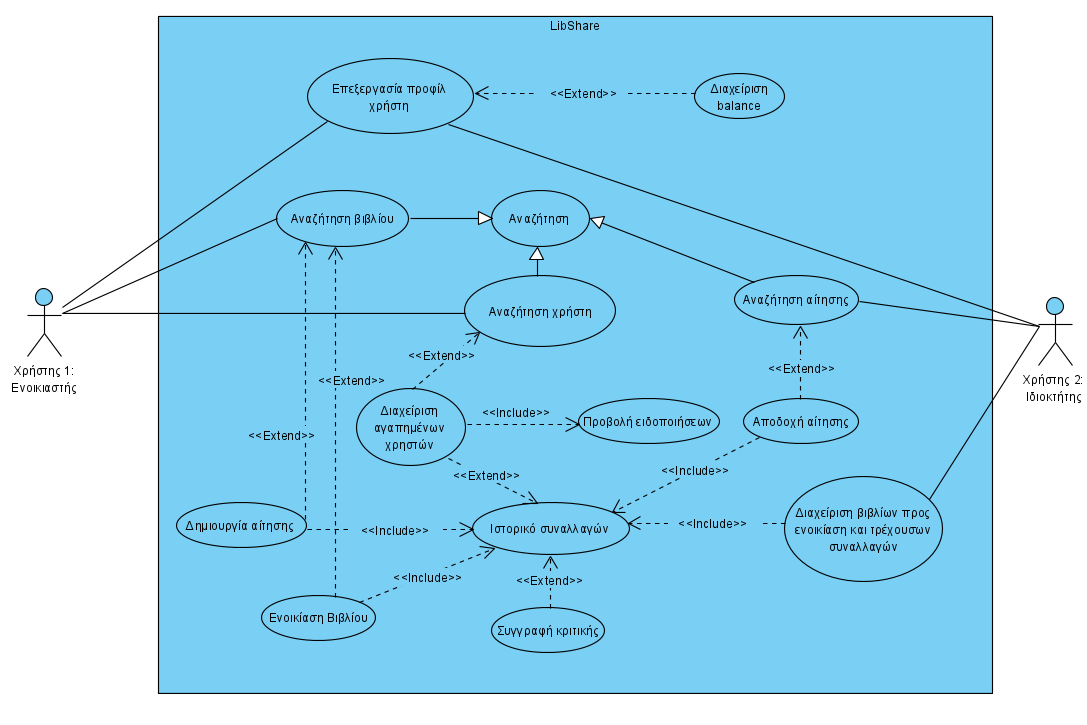
\includegraphics[width=\textwidth]{Use-case Diagram.png}}
	\caption{Use Case Diagram}
	\label{Use Case Diagram}
\end{figure}


\section{Ροές των Use Cases}
\label{Ροές των Use Cases}

\subsection{Αναζήτηση βιβλίων / χρήστη / αιτήσεων}

\subsubsection*{Βασική Ροή <<Αναζήτηση βιβλίων / χρήστη / αιτήσεων>>: Αναζήτηση βιβλίων με δια ζώσης συναλλαγή:}
\begin{enumerate}
    \item Ο χρήστης επιλέγει φίλτρο αναζήτησης "βιβλία", με τύπο συναλλαγής "δια ζώσης" και εισάγει ένα κείμενο αναζήτησης (μπορεί να είναι και τίτλος βιβλίου και όνομα συγγραφέα).
        \label{Επιλογή τύπου αναζήτησης}
    \item Το σύστημα ελέγχει αν υπάρχουν διαθέσιμα βιβλία προς ενοικίαση που πληρούν το κείμενο αναζήτησης, το τύπο συναλλαγής και ο ιδιοκτήτης τους να μένει στην ίδια πόλη με τον χρήστη και βλέπει ότι υπάρχουν.
        \label{Ύπαρξη βιβλίου}
    \item Το σύστημα δείχνει τη λίστα με τα διαθέσιμα βιβλία στον χρήστη, περιέχοντας τους πλήρεις τίτλους, το όνομα συγγραφέα, τον εκδοτικό οίκο και έτος τύπωσης.
    \item Ο χρήστης επιλέγει ένα από τα βιβλία.
    \item Το σύστημα φορτώνει τη λίστα των ιδιοκτητών που προσφέρουν το βιβλίο που επιλέχθηκε και την προβάλλει στον χρήστη, μαζί με την τιμή του βιβλίου ανά μέρα, την πόλη που μένει ο κάθε χρήστης, το σκορ του (που προκύπτει από τα ratings άλλων χρηστών) και κουμπί που του επιτρέπει να δηλώσει προσφορά ενοικίασης του βιβλίου στον χρήστη αυτόν.
    \item Ο χρήστης μεταφέρεται στο use case "Ενοικίαση βιβλίου από άλλο χρήστη".
\end{enumerate}

\subsubsection*{Εναλλακτική Ροή 1: Αναζήτηση χρήστη - Αυτός υπάρχει:}
\begin{enumerate}
    \item[\ref{Επιλογή τύπου αναζήτησης}.α.1.] Ο χρήστης επιλέγει φίλτρο αναζήτησης "χρήστης" και εισάγει ένα κείμενο αναζήτησης (το username του χρήστη που αναζητεί).
    \item[\ref{Επιλογή τύπου αναζήτησης}.α.2.] Το σύστημα ελέγχει αν υπάρχει άλλος χρήστης με το όνομα που ζήτησε ο χρήστης και βλέπει ότι υπάρχει.
    \item[\ref{Επιλογή τύπου αναζήτησης}.α.3.] Το σύστημα προβάλλει στον χρήστη το προφίλ του χρήστη που αναζήτησε, δηλαδή το username, το rating του, την τοποθεσία που μένει και το description που έχει ορίσει για τον λογαριασμό του. Επίσης προβάλλει ένα κουμπί προσθήκης χρήστη στη λίστα των αγαπημένων (το οποίο χρησιμοποιείται για το use case των notifications και αγαπημένων).
    \item[\ref{Επιλογή τύπου αναζήτησης}.α.4.] Ο χρήστης μεταφέρεται στο use case "Επεξεργασία λίστας αγαπημένων και χρήση συστήματος ειδοποιήσεων".
\end{enumerate}

\subsubsection*{Εναλλακτική Ροή 2: Αναζήτηση χρήστη - Αυτός δεν υπάρχει:}
\begin{enumerate}
    \item[\ref{Επιλογή τύπου αναζήτησης}.β.1.] Ο χρήστης επιλέγει φίλτρο αναζήτησης "χρήστης" και εισάγει ένα κείμενο αναζήτησης (το username του χρήστη που αναζητεί).
    \item[\ref{Επιλογή τύπου αναζήτησης}.β.2.] Το σύστημα ελέγχει αν υπάρχει άλλος χρήστης με το όνομα που ζήτησε ο χρήστης και βλέπει ότι δεν υπάρχει.
    \item[\ref{Επιλογή τύπου αναζήτησης}.β.3.] Το σύστημα ενημερώνει τον χρήστη ότι ο χρήστης που αναζητεί δεν υπάρχει.
\end{enumerate}

\subsubsection*{Εναλλακτική Ροή 3: Αναζήτηση αίτησης με δια ζώσης συναλλαγή - Αυτή υπάρχει:}
\begin{enumerate}
    \item[\ref{Επιλογή τύπου αναζήτησης}.γ.1.] Ο χρήστης επιλέγει φίλτρο αναζήτησης "αιτήσεις", με τύπο συναλλαγής "δια ζώσης", και εισάγει ένα κείμενο αναζήτησης (το όνομα του βιβλίου για το οποίο αναζητά αν υπάρχουν αιτήσεις).
    \item[\ref{Επιλογή τύπου αναζήτησης}.γ.2.] Το σύστημα ελέγχει αν υπάρχει αίτηση που να πληρεί τα κριτήρια αναζήτησης που ζήτησε ο χρήστης και διαπιστώνει ότι υπάρχει.
    \item[\ref{Επιλογή τύπου αναζήτησης}.γ.3.] Το σύστημα δείχνει τη λίστα με τα βιβλία για τα οποία υπάρχουν αιτήσεις που πληρούν τα κριτήρια αναζήτησης στον χρήστη, περιέχοντας τους πλήρεις τίτλους, το όνομα συγγραφέα, τον εκδοτικό οίκο και έτος τύπωσης.
    \item[\ref{Επιλογή τύπου αναζήτησης}.γ.4.] Ο χρήστης επιλέγει ένα από τα βιβλία.
    \item[\ref{Επιλογή τύπου αναζήτησης}.γ.5.] Το σύστημα φορτώνει τη λίστα των χρηστών που έχουν κάνει αίτηση για το βιβλίο που επιλέχθηκε και την προβάλλει στον χρήστη, μαζί με την τιμή που προτίθενται να πληρώσει ο κάθε χρήστης για το βιβλίο ανά μέρα, την πόλη που μένει ο καθένας, το σκορ τους και κουμπί που του επιτρέπει να κάνει προσφορά εκπλήρωσης της αίτησης.
    \item[\ref{Επιλογή τύπου αναζήτησης}.γ.6.] Ο χρήστης μεταφέρεται στο use case "Ενοικίαση βιβλίου σε άλλο χρήστη" (από τη μεριά του ιδιοκτήτη).
\end{enumerate}

\subsubsection*{Εναλλακτική Ροή 4: Αναζήτηση αίτησης με δια ζώσης συναλλαγή - Αυτή δεν υπάρχει:}
\begin{enumerate}
    \item[\ref{Επιλογή τύπου αναζήτησης}.δ.1.] Ο χρήστης επιλέγει φίλτρο αναζήτησης "αιτήσεις", με τύπο συναλλαγής "δια ζώσης", και εισάγει ένα κείμενο αναζήτησης (το όνομα του βιβλίου για το οποίο αναζητά αν υπάρχουν αιτήσεις).
    \item[\ref{Επιλογή τύπου αναζήτησης}.δ.2.] Το σύστημα ελέγχει αν υπάρχει αίτηση για το βιβλίο που αναζήτησε ο χρήστης και διαπιστώνει ότι δεν υπάρχει.
    \item[\ref{Επιλογή τύπου αναζήτησης}.δ.3.] Το σύστημα ενημερώνει τον χρήστη ότι δεν υπάρχει αίτηση που να πληρεί τα κριτήρια αναζήτησης.
\end{enumerate}

\subsubsection*{Εναλλακτική Ροή 5: Αναζήτηση βιβλίου - Ταχυδρομική συναλλαγή}
\begin{enumerate}
    \item[\ref{Επιλογή τύπου αναζήτησης}.ε.1.] Ο χρήστης επιλέγει φίλτρο αναζήτησης "βιβλία", με τύπο συναλλαγής "ταχυδρομικώς" και εισάγει ένα κείμενο αναζήτησης (μπορεί να είναι και τίτλος βιβλίου και όνομα συγγραφέα).
    \item[\ref{Επιλογή τύπου αναζήτησης}.ε.2.] Η περίπτωση χρήσης συνεχίζεται από το βήμα \ref{Ύπαρξη βιβλίου} της βασικής ροής μέχρι και το βήμα 5 (δεν θέλω να το αντιγράψω εδώ).
    \item[\ref{Επιλογή τύπου αναζήτησης}.ε.3.] Ο χρήστης μεταφέρεται στο use case "Ενοικίαση βιβλίου από άλλο χρήστη".
\end{enumerate}

\subsubsection*{Εναλλακτική Ροή 6: Αναζήτηση βιβλίου - Αυτό δεν υπάρχει:}
\begin{enumerate}
    \item[\ref{Ύπαρξη βιβλίου}.1.] Το σύστημα ελέγχει αν υπάρχουν διαθέσιμα βιβλία προς ενοικίαση που να πληρούν το κείμενο αναζήτησης και βλέπει ότι δεν υπάρχουν.
    \item[\ref{Ύπαρξη βιβλίου}.2.] Το σύστημα ενημερώνει τον χρήστη ότι δεν υπάρχουν διαθέσιμα βιβλία που να πληρούν τα κριτήρια αναζήτησης. 
\end{enumerate}

\subsubsection*{Εναλλακτική Ροή 7: Αναζήτηση αίτησης - Ταχυδρομική συναλλαγή}
\begin{enumerate}
    \item[\ref{Επιλογή τύπου αναζήτησης}.γ.1.α.1.] Ο χρήστης επιλέγει φίλτρο αναζήτησης "αιτήσεις", με τύπο συναλλαγής "ταχυδρομικώς", και εισάγει ένα κείμενο αναζήτησης (το όνομα του βιβλίου για το οποίο αναζητά αν υπάρχουν αιτήσεις).
    \item[\ref{Επιλογή τύπου αναζήτησης}.γ.1.α.2.] Η περίπτωση χρήσης συνεχίζεται από το βήμα 1.γ.1.2 της βασικής ροής, μέχρι το βήμα 1.γ.1.5 (δεν θέλω να το αντιγράψω εδώ).
    \item[\ref{Επιλογή τύπου αναζήτησης}.γ.1.α.3.] Ο χρήστης μεταφέρεται στο use case "Ενοικίαση βιβλίου από άλλο χρήστη" (από τη μεριά του ιδιοκτήτη).
\end{enumerate}

\subsection{Ενοικίαση βιβλίου από άλλο χρήστη}
\label{Rental Use Case}
\subsubsection*{Βασική Ροή <<Ενοικίαση βιβλίου από άλλο χρήστη>>:}
\begin{enumerate}
    \item Ο ενοικιαστής κάνει προσφορά ενοικίασης στον ιδιοκτήτη που επέλεξε για το βιβλίο που αναζήτησε.
        \label{Επιλογή τρόπου συναλλαγής}
    \item Το σύστημα επιβεβαιώνει ότι ο ενοικιαστής έχει αρκετά χρήματα στο λογαριασμό του για να καλύψει το "ποσό ασφαλείας" που θα δεσμευτεί αργότερα από τον λογαριασμό του.
        \label{Έλεγχος ποσού ασφαλείας}
    \item Το σύστημα επιβεβαιώνει ότι η προσφορά ενοικίασης έχει γίνει αποδεκτή από τον ιδιοκτήτη.
        \label{Αποδοχή ή απόρριψη συναλλαγής}
    \item Το σύστημα εμφανίζει στοιχεία επικοινωνίας του ιδιοκτήτη στον ενοικιαστή και αντίστροφα.
    \item Ο ενοικιαστής, αφού βρεθεί με τον ιδιοκτήτη δια ζώσης και παραλάβει το βιβλίο ή το βιβλίο φτάσει σε αυτόν μέσω ταχυδρομείου, ενημερώνει το σύστημα ότι έχει κατοχή του βιβλίου. Ο ιδιοκτήτης επίσης ενημερώνει το σύστημα.
    \item Το σύστημα ελέγχει αν έλαβε ενημέρωση κατοχής του βιβλίου και από τον ενοικιαστή και από τον ιδιοκτήτη.
        \label {Δεν ενημερώνεται η κατοχή}
    \item Το σύστημα δεσμεύει "ποσό ασφαλείας" από τον λογαριασμό του ενοικιαστή, και αρχίζει να τον χρεώνει αυτόματα μέρα με τη μέρα.
        \label{Τέλος dispute resolved - Τέλος χρημάτων}
    \item Ο ενοικιαστής, αφού τελειώσει το βιβλίο, βρίσκεται πάλι με τον ιδιοκτήτη και του παραχωρεί το βιβλίο ή αποστέλλει πίσω το βιβλίο ταχυδρομικώς, και όταν αυτό βρίσκεται πλέον πίσω στην κατοχή του ιδιοκτήτη ενημερώνουν και οι δύο το σύστημα για την επιτυχή επιστροφή του βιβλίου.
        \label{Επιστροφή βιβλίου - Τέλος λεφτά δεν φτάνουν}
    \item Το σύστημα ελέγχει ότι έχει λάβει ενημέρωση επιστροφής βιβλίου και από τα δύο μέλη. 
    \item Το σύστημα σταματάει να χρεώνει τον ενοικιαστή και του επιστρέφει το "ποσό ασφαλείας". Επίσης καταγράφει την λήξη της συναλλαγής και την αποθηκεύει στο ιστορικό συναλλαγών των δύο χρηστών.
        \label{Τέλος ενοικίασης}
\end{enumerate}

\subsubsection*{Εναλλακτική Ροή 1: Ο ενοικιαστής αποδέχεται μια προσφορά εκπλήρωσης αίτησης:}
\begin{enumerate}
    \item[1.1.] Ο ενοικιαστής αποδέχεται μια προσφορά εκπλήρωσης αίτησης που του έκανε άλλος χρήστης.
    \item[1.2.] Η περίπτωση χρήσης συνεχίζεται από το βήμα 4 της βασικής ροής.
\end{enumerate}

\subsubsection*{Εναλλακτική Ροή 2: Ο ενοικιαστής δεν έχει αρκετό υπόλοιπο για να καλύψει το "ποσό ασφαλείας":}
\begin{enumerate}
    \item[\ref{Έλεγχος ποσού ασφαλείας}.1.] Το σύστημα παρατηρεί ότι ο ενοικιαστής δεν έχει αρκετό χρηματικό ποσό στο λογαριασμό για να καλύψει το "ποσό ασφαλείας".
    \item[\ref{Έλεγχος ποσού ασφαλείας}.2.] Ο ενοικιαστής ενημερώνεται από το σύστημα ότι δεν έχει αρκετά χρήματα στον λογαριασμό του και να προσθέσει αν θέλει να κάνει την προσφορά ενοικίασης.
\end{enumerate}

\subsubsection*{Εναλλακτική Ροή 3: Η συναλλαγή απορρίπτεται από τον ιδιοκτήτη:}
\begin{enumerate}
    \item[\ref{Αποδοχή ή απόρριψη συναλλαγής}.1.] Το σύστημα παρατηρεί ότι η προσφορά ενοικίασης απορρίπτεται από τον ιδιοκτήτη.
    \item[\ref{Αποδοχή ή απόρριψη συναλλαγής}.2.] Ο ενοικιαστής ενημερώνεται από το σύστημα ότι η αίτησή του απορρίφθηκε από τον ιδιοκτήτη.
    \item[\ref{Αποδοχή ή απόρριψη συναλλαγής}.3.] Η συναλλαγή ολοκληρώνεται και αποθηκεύεται (ως ακυρωμένη) στο ιστορικό συναλλαγών των δύο χρηστών από το σύστημα.
\end{enumerate}

\subsubsection*{Εναλλακτική Ροή 4: Δεν ενημερώνεται και από τους δύο η κατάσταση κατοχής - Επίλυση προβλήματος:}
\begin{enumerate}
    \item[\ref{Δεν ενημερώνεται η κατοχή}.α.1.] Το σύστημα λαμβάνει ενημέρωση αλλαγής κατοχής από τον ιδιοκτήτη και όχι από τον ενοικιαστή.
    \item[\ref{Δεν ενημερώνεται η κατοχή}.α.2.] Το σύστημα ενημερώνει και τα δύο μέλη να επικοινωνήσουν μεταξύ τους και αν δεν λυθεί το θέμα να επικοινωνήσουν με την υποστήριξη πελατών.
    \item[\ref{Δεν ενημερώνεται η κατοχή}.α.3.] Το σύστημα λαμβάνει ενημέρωση κατοχής και από τον ενοικιαστή.
    \item[\ref{Δεν ενημερώνεται η κατοχή}.α.4.] Η περίπτωση χρήσης συνεχίζεται από το βήμα \ref{Τέλος dispute resolved - Τέλος χρημάτων} της βασικής ροής.
\end{enumerate}

\subsubsection*{Εναλλακτική Ροή 5: Δεν ενημερώνεται και από τους δύο η κατάσταση κατοχής - Επίλυση από υποστήριξη πελατών:}
\begin{enumerate}
    \item[\ref{Δεν ενημερώνεται η κατοχή}.β.1.] Το σύστημα λαμβάνει ενημέρωση αλλαγής κατοχής από τον ιδιοκτήτη και όχι από τον ενοικιαστή.
    \item[\ref{Δεν ενημερώνεται η κατοχή}.β.2.] Το σύστημα ενημερώνει και τα δύο μέλη να επικοινωνήσουν μεταξύ τους.
    \item[\ref{Δεν ενημερώνεται η κατοχή}.β.3.] Το σύστημα δεν λαμβάνει ενημέρωση κατοχής και από τον ενοικιαστή.
    \item[\ref{Δεν ενημερώνεται η κατοχή}.β.4.] Το σύστημα ενημερώνει και τα δύο μέλη να επικοινωνήσουν με την υποστήριξη πελατών.
\end{enumerate}

\subsubsection*{Εναλλακτική Ροή 6: Δεν ενημερώνεται και από τους δύο η κατάσταση επιστροφής - Επίλυση προβλήματος:}
\begin{enumerate}
    \item[\ref{Επιστροφή βιβλίου - Τέλος λεφτά δεν φτάνουν}.α.1.] Το σύστημα λαμβάνει ενημέρωση επιστροφής από τον ιδιοκτήτη και όχι από τον ενοικιαστή, ή αντίστροφα.
    \item[\ref{Επιστροφή βιβλίου - Τέλος λεφτά δεν φτάνουν}.α.2.] Το σύστημα ενημερώνει και τα δύο μέλη να επικοινωνήσουν μεταξύ τους και αν δεν λυθεί το θέμα να επικοινωνήσουν με την υποστήριξη πελατών.
    \item[\ref{Επιστροφή βιβλίου - Τέλος λεφτά δεν φτάνουν}.α.3.] Το σύστημα λαμβάνει ενημέρωση επιστροφής και από τον ενοικιαστή.
    \item[\ref{Επιστροφή βιβλίου - Τέλος λεφτά δεν φτάνουν}.α.4.] Η περίπτωση χρήσης συνεχίζεται από το βήμα \ref{Τέλος ενοικίασης}.
\end{enumerate}

\subsubsection*{Εναλλακτική Ροή 7: Δεν ενημερώνεται και από τους δύο η κατάσταση επιστροφής - Επίλυση από υποστήριξη πελατών:}
\begin{enumerate}
    \item[\ref{Επιστροφή βιβλίου - Τέλος λεφτά δεν φτάνουν}.β.1.] Το σύστημα λαμβάνει ενημέρωση επιστροφής από τον ιδιοκτήτη και όχι από τον ενοικιαστή, ή αντίστροφα.
    \item[\ref{Επιστροφή βιβλίου - Τέλος λεφτά δεν φτάνουν}.β.2.] Το σύστημα ενημερώνει και τα δύο μέλη να επικοινωνήσουν μεταξύ τους.
    \item[\ref{Επιστροφή βιβλίου - Τέλος λεφτά δεν φτάνουν}.β.3.] Το σύστημα δεν λαμβάνει ενημέρωση επιστροφής και από ενοικιαστή.
    \item[\ref{Επιστροφή βιβλίου - Τέλος λεφτά δεν φτάνουν}.β.4.] Το σύστημα ενημερώνει και τα δύο μέλη να επικοινωνήσουν με την υποστήριξη πελατών.
\end{enumerate}

\subsubsection*{Εναλλακτική Ροή 8: Τέλος χρημάτων ενοικιαστή - Μετέπειτα προσθήκη απαραίτητου ποσού:}
\begin{enumerate}
    \item[\ref{Τέλος dispute resolved - Τέλος χρημάτων}.α.1.] Το σύστημα αντιλαμβάνεται ότι έχουν τελειώσει τα χρήματα του ενοικιαστή.
    \item[\ref{Τέλος dispute resolved - Τέλος χρημάτων}.α.2.] Το σύστημα ζητάει από τον ενοικιαστή να προσθέσει παραπάνω χρήματα στον λογαριασμό του.
    \item[\ref{Τέλος dispute resolved - Τέλος χρημάτων}.α.3.] Ο ενοικιαστής προσθέτει παραπάνω χρήματα στον λογαριασμό του.
    \item[\ref{Τέλος dispute resolved - Τέλος χρημάτων}.α.4.] Το σύστημα αντιλαμβάνεται ότι προστέθηκαν παραπάνω χρήματα και χρεώνει από τον ενοικιαστή το ποσό που οφείλει, μαζί με 20\% επιτόκιο.
    \item[\ref{Τέλος dispute resolved - Τέλος χρημάτων}.α.5.] Η περίπτωση χρήσης συνεχίζεται από το βήμα \ref{Επιστροφή βιβλίου - Τέλος λεφτά δεν φτάνουν} της βασικής ροής.
\end{enumerate}

\subsubsection*{Εναλλακτική Ροή 9: Τέλος χρημάτων ενοικιαστή - Δεν προστίθεται το απαραίτητο ποσό:}
\begin{enumerate}
    \item[\ref{Τέλος dispute resolved - Τέλος χρημάτων}.β.1.] Το σύστημα αντιλαμβάνεται ότι έχουν τελειώσει τα χρήματα του ενοικιαστή.
    \item[\ref{Τέλος dispute resolved - Τέλος χρημάτων}.β.2.] Το σύστημα ζητάει από τον ενοικιαστή να προσθέσει παραπάνω χρήματα στον λογαριασμό του.
    \item[\ref{Τέλος dispute resolved - Τέλος χρημάτων}.β.3.] Το σύστημα αντιλαμβάνεται μετά από ένα χρονικό διάστημα 2 εβδομάδων ότι ο χρήστης δεν έχει προσθέσει το ποσό που οφείλει στον λογαριασμό του.
    \item[\ref{Τέλος dispute resolved - Τέλος χρημάτων}.β.4.] Το σύστημα προσφέρει αυτόματα το "ποσό ασφαλείας" στον ιδιοκτήτη και απενεργοποιεί τη δυνατότητα του ενοικιαστή να νοικιάσει άλλο βιβλίο, μέχρι να πληρώσει το χρωστούμενο ποσό.
\end{enumerate}

\subsection{Ενοικίαση βιβλίου σε άλλο χρήστη (μεριά ιδιοκτήτη)}
\subsubsection*{Βασική Ροή <<Ενοικίαση βιβλίου σε άλλο χρήστη (μεριά ιδιοκτήτη)>>:}
\begin{enumerate}
    \item Ο ιδιοκτήτης αποδέχεται την προσφορά ενοικίασης βιβλίου που του έκανε ένας άλλος χρήστης.
    \item Το σύστημα καταγράφει ότι η προσφορά ενοικίασης έχει γίνει αποδεκτή από τον ιδιοκτήτη. 
    \item Το σύστημα αφαιρεί ένα από το διαθέσιμο υπόλοιπο για το συγκεκριμένου βιβλίου που προφέρει ο ιδιοκτήτης προς ενοικίαση (επειδή μπορεί ο ιδιοκτήτης να έχει πολλά αντίγραφα από το ίδιο βιβλίο που προσφέρει για ενοικίαση). Το διαθέσιμο υπόλοιπο μετά την αφαίρεση είναι μεγαλύτερο του μηδέν.
    \item Το σύστημα εμφανίζει στοιχεία επικοινωνίας του ιδιοκτήτη στον ενοικιαστή και αντίστροφα.
    \item Ο ιδιοκτήτης βρίσκεται με τον ενοικιαστή δια ζώσης και του δίνει το βιβλίο, ή στέλνει το βιβλίο ταχυδρομικώς (ανάλογα τον τύπο συναλλαγής που επιλέχθηκε) και ενημερώνει τη πλατφόρμα (δήλωση αλλαγής κατοχής) όταν ο ενοικιαστής πλέον έχει το βιβλίο (αφού του το δώσει ή αφού φτάσει σύμφωνα με το tracking number του ταχυδρομείου αντίστοιχα).
    \item Το σύστημα ελέγχει ότι έχει λάβει ενημέρωση κατοχής του βιβλίου και από τους δύο χρήστες. 
    \item Το σύστημα δεσμεύει το "ποσό ασφαλείας" από τον ενοικιαστή και αρχίζει να τον χρεώνει μέρα με τη μέρα, μεταφέροντας καθημερινά το ποσό χρέωσης από τον λογαριασμό του ενοικιαστή στον λογαριασμό του ιδιοκτήτη.
    \item Ο ιδιοκτήτης, αφού λάβει πίσω το βιβλίο από συνάντηση δια ζώσης ή ταχυδρομικώς, ενημερώνει την πλατφόρμα ότι το βιβλίο επιστράφηκε (δήλωση επιστροφής).
    \item Το σύστημα ελέγχει ότι έχει λάβει ενημέρωση επιστροφής βιβλίου και από τα δύο μέλη.
    \item Το σύστημα σταματάει να χρεώνει τον ενοικιαστή και του επιστρέφει το "ποσό ασφαλείας". Επίσης καταγράφει την λήξη της συναλλαγής και την αποθηκεύει στο ιστορικό συναλλαγών των δύο χρηστών.
\end{enumerate}

\subsubsection*{Εναλλακτική Ροή 1: Ο ιδιοκτήτης κάνει προσφορά εκπλήρωσης αίτησης ενός άλλου χρήστη:}
\begin{enumerate}
    \item[1.α.1.] Ο ιδιοκτήτης κάνει προσφορά εκπλήρωσης αίτησης στον ενοικιαστή που επέλεξε για την αίτηση που αναζήτησε.
    \item[1.α.2.] Το σύστημα επιβεβαιώνει ότι ο ενοικιαστής έχει αρκετά χρήματα στο λογαριασμό του για να καλύψει το "ποσό ασφαλείας" που θα δεσμευτεί αργότερα από τον λογαριασμό του.
    \item[1.α.3.] Το σύστημα επιβεβαιώνει ότι η προσφορά εκπλήρωσης αίτησης έχει γίνει αποδεκτή από τον ενοικιαστή.
    \item[1.α.4.] Η περίπτωση χρήσης συνεχίζεται από το βήμα 4 της βασικής ροής.
\end{enumerate}

\subsubsection*{Εναλλακτική Ροή 2: Η συναλλαγή απορρίπτεται από τον ιδιοκτήτη:}
\begin{enumerate}
    \item[1.β.1.] Ο ιδιοκτήτης απορρίπτει την προσφορά ενοικίασης βιβλίου που του έκανε ένας άλλος χρήστης.
    \item[1.β.2.] Το σύστημα παρατηρεί ότι η προσφορά ενοικίασης απορρίπτεται από τον ιδιοκτήτη.
    \item[1.β.3.] Η συναλλαγή ολοκληρώνεται και αποθηκεύεται (ως ακυρωμένη) στο ιστορικό συναλλαγών των δύο χρηστών από το σύστημα.
\end{enumerate}

\subsubsection*{Εναλλακτική Ροή 3: Το διαθέσιμο υπόλοιπο καταλήγει να είναι μηδέν:}
\begin{enumerate}
    \item[3.1.] Το σύστημα αφαιρεί ένα από το διαθέσιμο υπόλοιπο για το συγκεκριμένου βιβλίου που προφέρει ο ιδιοκτήτης προς ενοικίαση (επειδή μπορεί ο ιδιοκτήτης να έχει πολλά αντίγραφα από το ίδιο βιβλίο που προσφέρει για ενοικίαση). Το διαθέσιμο υπόλοιπο μετά την αφαίρεση είναι ίσο με μηδέν.
    \item[3.2.] Το σύστημα δεν δείχνει το βιβλίο ως διαθέσιμο πλέον από τον συγκεκριμένο ιδιοκτήτη και δεν μπορούν να γίνουν νέες αιτήσεις ενοικιάσεως.
    \item[3.3.] Η περίπτωση χρήσης συνεχίζεται από το βήμα 4 της βασικής ροής.
\end{enumerate}

\subsubsection*{Εναλλακτική Ροή 4: Δεν ενημερώνεται και από τους δύο η κατάσταση κατοχής - Επίλυση προβλήματος:}
\begin{enumerate}
    \item[6.α.1.] Το σύστημα λαμβάνει ενημέρωση αλλαγής κατοχής από τον ενοικιαστή και όχι από τον ιδιοκτήτη.
    \item[6.α.2.] Το σύστημα ενημερώνει και τα δύο μέλη να επικοινωνήσουν μεταξύ τους και αν δεν λυθεί το θέμα να επικοινωνήσουν με την υποστήριξη πελατών.
    \item[6.α.3.] Το σύστημα λαμβάνει ενημέρωση κατοχής και από ιδιοκτήτη.
    \item[6.α.4.] Η περίπτωση χρήσης συνεχίζεται από το βήμα 7 της βασικής ροής.
\end{enumerate}

\subsubsection*{Εναλλακτική Ροή 5: Δεν ενημερώνεται και από τους δύο η κατάσταση κατοχής - Επίλυση από υποστήριξη πελατών:}
\begin{enumerate}
    \item[6.β.1.] Το σύστημα λαμβάνει ενημέρωση αλλαγής κατοχής από τον ενοικιαστή και όχι από τον ιδιοκτήτη.
    \item[6.β.2.] Το σύστημα ενημερώνει και τα δύο μέλη να επικοινωνήσουν μεταξύ τους.
    \item[6.β.3.] Το σύστημα δεν λαμβάνει ενημέρωση κατοχής και από τον ιδιοκτήτη.
    \item[6.β.4.] Το σύστημα ενημερώνει και τα δύο μέλη να επικοινωνήσουν με την υποστήριξη πελατών.
\end{enumerate}

\subsubsection*{Εναλλακτική Ροή 6: Δεν ενημερώνεται και από τους δύο η κατάσταση επιστροφής - Επίλυση προβλήματος:}
\begin{enumerate}
    \item[9.α.1.] Το σύστημα λαμβάνει ενημέρωση επιστροφής από τον ενοικιαστή και όχι από τον ιδιοκτήτη του βιβλίου.
    \item[9.α.2.] Το σύστημα ενημερώνει και τα δύο μέλη να επικοινωνήσουν μεταξύ τους και αν δεν λυθεί το θέμα να επικοινωνήσουν με την υποστήριξη πελατών.
    \item[9.α.3.] Το σύστημα λαμβάνει ενημέρωση επιστροφής και από τον ιδιοκτήτη.
    \item[9.α.4.] Η περίπτωση χρήσης συνεχίζεται από το βήμα 10.
\end{enumerate}

\subsubsection*{Εναλλακτική ροή 7: Ο χρήστης απορρίπτει την προσφορά ενοικίασης του άλλου χρήστη:}
\begin{enumerate}
    \item [6.1] Ο χρήστης απορρίπτει την προσφορά.
    \item [6.2] Το σύστημα ανανεώνει το status της προσφοράς ως "Απόρριψη από ιδιοκτήτη" και την μεταφέρει στα ιστορικά των δύο χρηστών.
    \item [6.3] Το σύστημα ενημερώνει τον χρήστη ότι η απόρριψη καταγράφτηκε.
\end{enumerate}


\subsubsection*{Εναλλακτική Ροή 8: Δεν ενημερώνεται και από τους δύο η κατάσταση επιστροφής - Επίλυση από υποστήριξη πελατών:}
\begin{enumerate}
    \item[9.β.1.] Το σύστημα λαμβάνει ενημέρωση επιστροφής από τον ενοικιαστή και όχι από τον ιδιοκτήτη του βιβλίου.
    \item[9.β.2.] Το σύστημα ενημερώνει και τα δύο μέλη να επικοινωνήσουν μεταξύ τους.
    \item[9.β.3.] Το σύστημα δεν λαμβάνει ενημέρωση επιστροφής και από τον ιδιοκτήτη.
    \item[9.β.4.] Το σύστημα ενημερώνει και τα δύο μέλη να επικοινωνήσουν με την υποστήριξη πελατών.
\end{enumerate}

\subsection{Διαχείριση των βιβλίων που προσφέρει ο χρήστης προς ενοικίαση από άλλους}

\subsubsection*{Βασική ροή <<Διαχείριση των βιβλίων που προσφέρει ο χρήστης \\προς ενοικίαση από άλλους>>: Προσθήκη και ενοικίαση βιβλίου από άλλον χρήστη:}
\begin{enumerate}
    \item Ο χρήστης επιλέγει να προβάλλει τη λίστα των βιβλίων που προσφέρει για ενοικίαση.
    \item Το σύστημα φορτώνει τη λίστα των βιβλίων και την εμφανίζει στον χρήστη.
    \item Το σύστημα δίνει στον χρήστη την επιλογή να προσθέσει βιβλία προς ενοικίαση, να αφαιρέσει και να επεξεργαστεί τις πληροφορίες και τη ποσότητά αυτών που προσφέρει ήδη.
    \item Ο χρήστης επιλέγει να προσθέσει ένα νέο βιβλίο προς ενοικίαση από τους υπόλοιπους χρήστες.
    \item Ο χρήστης συμπληρώνει τα στοιχεία του βιβλίου (τίτλος, συγγραφέας, εκδοτικός οίκος και χρονολογία τύπωσης, κατηγορίες στις οποίες ανήκει το βιβλίο, τρόπος παράδοσης, τιμή, ποσότητα ίδιων βιβλίων) και ολοκληρώνει την προσθήκη.
    \item Το σύστημα καταγράφει τα στοιχεία του βιβλίου και ολοκληρώνει την προσθήκη.
    \item Το σύστημα ενημερώνει τον χρήστη ότι η προσθήκη έγινε με επιτυχία.
\end{enumerate}

\subsubsection*{Εναλλακτική ροή 1: Ο χρήστης δεν έχει εισάγει προηγουμένως βιβλία προς ενοικίαση από άλλους χρήστες:}
\begin{enumerate}
    \item [2.1.] Το σύστημα αντιλαμβάνεται ότι ο χρήστης δεν έχει προσθέσει προηγουμένως βιβλία προς ενοικίαση.
    \item [2.2.] Το σύστημα ενημερώνει αντίστοιχα τον χρήστη.
    \item [2.3.] Η ροή συνεχίζεται από το βήμα 3 της βασικής ροής.
\end{enumerate}

\subsubsection*{Εναλλακτική ροή 2: Ο χρήστης επιλέγει να αλλάξει τις πληροφορίες για βιβλίο που έχει ήδη προσθέσει:}
\begin{enumerate}
    \item [4.α.1.] Ο χρήστης επιλέγει να αλλάξει τις πληροφορίες για κάποιο από τα βιβλία που προσφέρει.
    \item [4.α.2.] Ο χρήστης επιλέγει το βιβλίο των οποίων τις πληροφορίες θέλει να αλλάξει.

    \item [4.α.3.] Ο χρήστης συμπληρώνει τις πληροφορίες που θέλει να ανανεώσει (τίτλος, συγγραφέας, εκδοτικός οίκος ή/και ποσότητα ίδιων βιβλίων), με εξαίρεση την ποσότητα για βιβλία που έχουν προηγούμενη ποσότητα μηδέν.

    \item [4.α.4.] Το σύστημα καταγράφει τις αλλαγές.
    \item [4.α.5.] Το σύστημα ενημερώνει τον χρήστη ότι οι αλλαγές έγιναν με επιτυχία.
\end{enumerate}

\subsubsection*{Εναλλακτική ροή 2: Ο χρήστης επιλέγει να αλλάξει την ποσότητα για ένα βιβλίο με προηγούμενη ποσότητα μηδέν:}
\begin{enumerate}
    \item [4.β.1.] Ο χρήστης επιλέγει να αλλάξει τις πληροφορίες για κάποιο από τα βιβλία που προσφέρει.
    \item [4.β.2.] Ο χρήστης επιλέγει το βιβλίο των οποίων τις πληροφορίες θέλει να αλλάξει.

    \item [4.β.3.] Ο χρήστης συμπληρώνει την ποσότητα που θέλει να ανανεώσει για ένα βιβλίο που είχε προηγουμένως ποσότητα μηδέν. 

    \item [4.β.4.] Το σύστημα καταγράφει τις αλλαγές.
    \item [4.β.5.] Το σύστημα κάνει ξανά το βιβλίο εμφανίσιμο στην αναζήτηση και δίνει πίσω την δυνατότητα ενοικίασής του από άλλους χρήστες.
    \item [4.β.6.] Το σύστημα ενημερώνει τον χρήστη ότι οι αλλαγές έγιναν με επιτυχία.
\end{enumerate}

\subsubsection*{Εναλλακτική ροή 3: Ο χρήστης επιλέγει να διαγράψει ένα από τα βιβλία από τη λίστα των βιβλίων που προσφέρει προς ενοικίαση:}
\begin{enumerate}
    \item [4.γ.1.] Ο χρήστης επιλέγει να αλλάξει διαγράψει ένα βιβλίο από τη λίστα αυτών που προσφέρει.
    \item [4.γ.2.] Ο χρήστης επιλέγει το βιβλίο που θέλει να διαγράψει.
    \item [4.γ.3.] Το σύστημα ζητάει επιβεβαίωση από τον χρήστη.
    \item [4.γ.4.] Ο χρήστης επιβεβαιώνει τη πρόθεση του να διαγράψει την εγγραφή.
    \item [4.γ.5.] Το σύστημα διαγράφει το βιβλίο από τη λίστα των διαθέσιμων βιβλίων του χρήστη.
    \item [4.γ.6.] Το σύστημα ενημερώνει τον χρήστη για την επιτυχή διαγραφή.
\end{enumerate}

\subsubsection*{Εναλλακτική ροή 4: Ο χρήστης επιλέγει να διαγράψει ένα από τα βιβλία από τη λίστα των βιβλίων που προσφέρει προς ενοικίαση, αλλά δεν επιβεβαιώνει:}
\begin{enumerate}
    \item [4.δ.1.] Ο χρήστης επιλέγει να αλλάξει διαγράψει ένα βιβλίο από τη λίστα αυτών που προσφέρει.
    \item [4.δ.2.] Ο χρήστης επιλέγει το βιβλίο που θέλει να διαγράψει.
    \item [4.δ.3.] Το σύστημα ζητάει επιβεβαίωση από τον χρήστη.
    \item [4.δ.4.] Ο χρήστης απορρίπτει την διαγραφή του βιβλίου.
    \item [4.δ.5.] Το σύστημα αντιλαμβάνεται την απόρριψη της διαγραφής.
    \item [4.δ.6.] Το σύστημα ενημερώνει τον χρήστη ότι η διαγραφή απορρίφθηκε.
\end{enumerate}

\subsection{Διαχείριση των αιτήσεων που έχει κάνει ο χρήστης}

\subsubsection*{Βασική ροή <<Διαχείριση των αιτήσεων που έχει κάνει ο χρήστης>>: Προσθήκη νέου αιτήματος:}
\begin{enumerate}
    \item Ο χρήστης επιλέγει να δει τη λίστα με τα αιτήματά του.
    \item Στον χρήστη εμφανίζεται η οθόνη με τα ήδη υπάρχοντα αιτήματά του μαζί με στοιχεία του καθενός από αυτά.
    \item Ο χρήστης πατάει την επιλογή προσθήκης καινούριου αιτήματος.
    \item Ο χρήστης εισάγει τα στοιχεία του βιβλίου τα οποία θέλει να αποκτήσει, προσθέτοντας την τιμή που προτίθεται να πληρώσει.
    \item Το σύστημα αναζητά αν αυτό το βιβλίο υπάρχει ήδη διαθέσιμο από κάποιον άλλο χρήστη που το προσφέρει ήδη στην πλατφόρμα.
    \item Το σύστημα προχωράει στην καταχώρηση του αιτήματος.
    \item Εμφανίζεται μήνυμα που γράφει “Επιτυχής καταχώρηση αιτήματος”.
    \item Ο χρήστης κλείνει το μήνυμα.
    \item Εμφανίζεται η λίστα των αιτημάτων ανανεωμένη με το νέο αίτημα.
\end{enumerate}

\subsubsection*{Εναλλακτική ροή 1: Ο χρήστης δεν έχει κάνει προηγούμενες αιτήσεις:}
\begin{enumerate}
    \item [2.1.] Το σύστημα αντιλαμβάνεται ότι o χρήστης δεν έχει κάνει καμία προηγούμενη αίτηση, οπότε εμφανίζεται μια άδεια οθόνη με μοναδική λειτουργία την προσθήκη αίτησης.
    \item [2.2.] Η ροή συνεχίζει από το βήμα 3 της βασικής ροής.
\end{enumerate}

\subsubsection*{Εναλλακτική ροή 2: Ο χρήστης αφαιρεί υπάρχουσα αίτηση:}
\begin{enumerate}
    \item [3.α.1.] Ο χρήστης επιλέγει την επιλογή remove request για μια αίτηση του το οποίο επέλεξε.
    \item [3.α.2.] Εμφανίζεται pop up το οποίο τον καλεί να επιβεβαιώσει την επιλογή του.
    \item [3.α.3.] Ο χρήστης πατάει ναι.
    \item [3.α.4.] Το request διαγράφεται.
    \item [3.α.5.] Εμφανίζεται πάλι η οθόνη των requests.
\end{enumerate}

\subsubsection*{Εναλλακτική ροή 3: Ο χρήστης κάνει edit υπάρχουσα αίτηση:}
\begin{enumerate}
    \item [3.β.1.] Ο χρήστης επιλέγει την επιλογή edit σε κάποια υπάρχουσα αίτηση.
    \item [3.β.2.] Εμφανίζεται μια καινούργια οθόνη με τα στοιχεία της αίτησης που επέλεξε.
    \item [3.β.3.] Επιλέγει το στοιχείο που θέλει να αλλάξει.
    \item [3.β.4.] Εμφανίζεται ένα pop up όπου συμπληρώνει την καινούργια τιμή.
    \item [3.β.5.] Πατάει OK.
    \item [3.β.6.] Επιστρέφει στην οθόνη με τα στοιχεία.
    \item [3.β.7.] Επιλέγει apply.
    \item [3.β.8.] Επιστρέφει την οθόνη με τα requests με τα ανανεωμένα στοιχεία.
\end{enumerate}

\subsubsection*{Εναλλακτική ροή 4: Το βιβλίο είναι ήδη διαθέσιμο προς ενοικίαση}
\begin{enumerate}
    \item[5.1.] Το σύστημα βρίσκει ότι βιβλίο το οποίο ο χρήστης αναζητούσε υπάρχει ήδη διαθέσιμο προς ενοικίαση από άλλον χρήστη.
    \item[5.2.] Εμφανίζει στο χρήστη την υπάρχουσα προσφορά με τα στοιχεία της και δυνατότητα ενοικίασης.
    \item[5.3.] Ο χρήστης επιχειρεί την ενοικίαση του βιβλίου.
    \item[5.4.] Το σύστημα μας προχωράει με τη διαδικασία του rent.
\end{enumerate}

\subsubsection*{Εναλλακτική ροή 5: Ο χρήσης δεν νοικιάζει το ήδη διαθέσιμο προς ενοικίαση βιβλίο}
\begin{enumerate}
    \item [5.3.1.] Ο χρήστης απορρίπτει την ενοικίαση του βιβλίου.
    \item [5.3.2.] Επιστρέφει στο βήμα 2 στη βασική ροή.
\end{enumerate}

\subsection{Εκπλήρωση αιτήσεων που έχουν κάνει άλλοι χρήστες}

\subsubsection*{Βασική ροή <<Εκπλήρωση αιτήσεων που έχουν κάνει άλλοι χρήστες>>: Εκπλήρωση αιτήματος:}
\begin{enumerate}
    \item Ο χρήστης επιλέγει να δει την οθόνη με τα υπάρχοντα request από την αναζήτηση.
    \item Το σύστημα ψάχνει για μη εκπληρωμένες αιτήσεις από άλλους χρήστες που να πληρούν τις συνθήκες αναζήτησης του χρήστη και βρίσκει ότι υπάρχουν.
    \item Το σύστημα εμφανίζει τις αιτήσεις αυτές στον χρήστη (μαζί με στοιχεία όπως το βιβλίο που ζητείται, τον συγγραφέα, την τιμή που προτίθεται να πληρώσει ο χρήστης, τον τρόπο συναλλαγής που θέλει και το σκορ του). 
    \item Ο αρχικός χρήστης επιλέγει να εκπληρώσει μια από τις αιτήσεις.
    \item Το σύστημα τον καλεί να επιβεβαιώσει την απόφαση του.
    \item Ο χρήστης επιβεβαιώνει.
    \item Ενεργοποιείται το πρωτόκολλο διαχείρισης συναλλαγών και δημιουργείται μια νέα συναλλαγή (στην οθόνη των τρεχουσών συναλλαγών) μεταξύ του αρχικού χρήστη και του χρήστη που έκανε την αίτηση, το οποίο είναι το ίδιο με τη διαδικασία στο use case του κεφαλαίου \ref{Rental Use Case} με τη διαφορά ότι ο χρήστης που έκανε την αίτηση είναι αυτός που πρέπει να επιβεβαιώσει το αρχικό αίτημα (δεν εξηγούμε ξανά όλη την όλη διαδικασία εφόσον κατά τα άλλα είναι η ίδια).
    \item Το σύστημα επιστρέφει το χρήστη στην οθόνη αναζήτησης requests.
\end{enumerate}

\subsubsection*{Εναλλακτική ροή 1: Το σύστημα βλέπει ότι δεν υπάρχει αίτημα που δεν είναι εκπληρωμένο:}
\begin{enumerate}
    \item [2.1.] Το σύστημα ψάχνει για μη εκπληρωμένες αιτήσεις από άλλους χρήστες που να πληρούν τις συνθήκες αναζήτησης του χρήστη και βρίσκει ότι δεν υπάρχουν.
    \item [2.2.] Το σύστημα ενημερώνει κατάλληλα τον χρήστη και του προτείνει να κάνει άλλη αναζήτηση.
\end{enumerate}

\subsubsection*{Εναλλακτική ροή 2: Ο χρήστης ακυρώνει την εκπλήρωση της αίτησης στο βήμα επιβεβαίωσης:}
\begin{enumerate}
    \item [6.1.] Ο χρήστης ακυρώνει την εξυπηρέτηση του request.
    \item [6.2.] To σύστημα επιστρέφει στην οθόνη requests.
\end{enumerate}

\subsection{Αξιολόγηση άλλων χρηστών μετά από την ολοκλήρωση συναλλαγής}

\subsubsection*{Βασική ροή <<Αξιολόγηση άλλων χρηστών μετά από την ολοκλήρωση συναλλαγής>>: Προσθήκη νέας αξιολόγησης με το προαιρετικό σχόλιο}
\begin{enumerate}
    \item Ο χρήστης επιλέγει μια ολοκληρωμένη συναλλαγή από το ιστορικό του, και διαλέγει να αξιολογήσει τον χρήστη με τον οποίο έκανε τη συναλλαγή.
    \item Εμφανίζεται μια επιλογή για αξιολόγηση της μορφής 1-5 αστεριών, μαζί με προαιρετική προσθήκη σχολίου με μήκος μέχρι 280 χαρακτήρες.
    \item Ο χρήστης συμπληρώνει την επιλογή για τα αστεράκια και προσθέτει και το προαιρετικό σχόλιο.
    \item Το σύστημα ελέγχει το μήκος του σχολίου και δεν επιτρέπει τον χρήστη να καταχωρήσει την αξιολόγησή του αν περνάει το μέγιστο επιτρεπτό μήκος.
    \item Ο χρήστης επιλέγει καταχωρήσει την αξιολόγησή του, έχοντας συμπληρώσει σχόλιο που τηρεί τον κανόνα μέγιστου μήκους.
    \item Το σύστημα ρωτάει τον χρήστη αν είναι σίγουρος πως θέλει να καταχωρήσει την αξιολόγησή του.
    \item Ο χρήστης επιβεβαιώνει την πρόθεσή του.
    \item Το σύστημα αποθηκεύει την αξιολόγηση.
    \item Εμφανίζεται μήνυμα που ενημερώνει τον χρήστη για την επιτυχία καταχώρησης της αξιολόγησης.
\end{enumerate}

\subsubsection*{Εναλλακτική ροή 1: Ο χρήστης κάνει αξιολόγηση χωρίς το προαιρετικό σχόλιο}
\begin{enumerate}
    \item [3.1.] Ο χρήστης συμπληρώνει την επιλογή για τα αστεράκια.
    \item [3.3.] Ο χρήστης καταχωρεί την αξιολόγησή του.
    \item [3.4.] Επιστροφή στο βήμα 6 της βασικής ροής.
\end{enumerate}

\subsubsection*{Εναλλακτική ροή 2: Ο χρήστης ακυρώνει την διαδικασία της αξιολόγησης}
\begin{enumerate}
    \item [7.1.] Ο χρήστης πατάει ακύρωση.
    \item [7.2.] Εμφανίζεται μήνυμα ακύρωσης αξιολόγησης.
\end{enumerate}

\subsection{Προβολή και Επεξεργασία στοιχείων λογαριασμού χρήστη:}

\subsubsection*{Βασική ροή <<Προβολής και επεξεργασίας στοιχείων λογαριασμού \\χρήστη>>:}
\begin{enumerate}
    \item Ο χρήστης επιλέγει να πάει στη σελίδα του προφίλ. 
    \item Το σύστημα φορτώνει τα στοιχεία του χρήστη (username, email, περιγραφή, τοποθεσία, κινητό τηλέφωνο και εικόνα χρήστη) και τα εμφανίζει στον χρήστη.
    \item Ο χρήστης επιλέγει να κάνει επεξεργασία των στοιχείων του και εισάγει νέα στοιχεία για αυτά που θέλει να αλλάξει (εκτός του password και της εικόνας χρήστη που αναλύονται σε εναλλακτική ροή και του email που δεν μπορεί να αλλάξει). 
    \item Το σύστημα ελέγχει αν τα στοιχεία έχουν τη σωστή μορφοποίηση, δηλαδή το username να έχει εύρος από 8-20 χαρακτήρες και δεν το έχει ήδη άλλος χρήστης, η περιγραφή μέχρι 150 χαρακτήρες, η τοποθεσία να είναι πραγματική και να υπάρχει στο χάρτη και το κινητό να είναι δεκαψήφιος αριθμός και βλέπει ότι οι κανόνες τηρούνται.
    \item Το σύστημα καταγράφει τις αλλαγές.
    \item Το σύστημα ενημερώνει τον χρήστη ότι έχουν ανανεωθεί τα στοιχεία του με μήνυμα και με email.
    \item Το σύστημα επιστρέφει τον χρήστη στην οθόνη του προφίλ του, όπου μπορεί να δει το ανανεωμένο προφίλ του.
\end{enumerate}

\subsubsection*{Εναλλακτική ροή 1: Τα νέα στοιχεία που εισάγει ο χρήστης δεν τηρούν τους κανόνες μορφοποίησης:}
\begin{enumerate}
    \item [4.α.1.] Το σύστημα ελέγχει τα νέα στοιχεία (username, περιγραφή, τοποθεσία, τηλέφωνο) και δεν τηρούνται οι προδιαγραφές.
    \item [4.α.2.] Το σύστημα εμφανίζει μήνυμα στον χρήστη ότι τα στοιχεία προς ανανέωση δεν έχουν κατάλληλη μορφοποίηση.
\end{enumerate}

\subsubsection*{Εναλλακτική ροή 2: Το νέο username χρησιμοποιείται ήδη από άλλον χρήστη:}
\begin{enumerate}
    \item [4.β.1.] Το σύστημα ελέγχει το νέο username και βλέπει ότι υπάρχει ήδη χρήστης με το username αυτό. 
    \item [4.β.2.] Το σύστημα εμφανίζει μήνυμα στον χρήστη ότι το username χρησιμοποιείται από άλλον χρήστη.  
\end{enumerate}

\subsubsection*{Εναλλακτική ροή 3: Ο χρήστης επιθυμεί αλλαγή του κωδικού:}
\begin{enumerate}
    \item [3.α.1.] Ο χρήστης επιλέγει αλλαγή του κωδικού του. 
    \item [3.α.2.] Το σύστημα του ζητάει να συμπληρώσει τον παλιό κωδικό του.
    \item [3.α.3.] Ο χρήστης συμπληρώνει τον παλιό κωδικό και το σύστημα ελέγχει αν είναι σωστός.
    \item [3.α.4.] Ο κωδικός είναι σωστός και το σύστημα ζητάει τον νέο κωδικό (2 φορές).
    \item [3.α.5.] Ο χρήστης εισάγει το νέο κωδικό 2 φορές.
    \item [3.α.6.] Το σύστημα αντιλαμβάνεται ότι ο χρήστης έχει εισάγει τον ίδιο νέο κωδικό και τις δύο φορές.
    \item [3.α.7.] Το σύστημα ανανεώνει τον κωδικό πρόσβασης του χρήστη.
    \item [3.α.8.] Το σύστημα ενημερώνει ότι έχει αλλάξει ο κωδικός.
    \item [3.α.9.] Το σύστημα επιστρέφει στο βήμα 5 της βασικής ροής.
\end{enumerate}

\subsubsection*{Εναλλακτική ροή 4: Ο παλιός κωδικός κατά την αλλαγή κωδικού δεν είναι σωστός:}
\begin{enumerate}
    \item [3.β.1.] Ο χρήστης επιλέγει αλλαγή του κωδικού του.
    \item [3.β.2.] Το σύστημα του ζητάει να συμπληρώσει τον παλιό κωδικό του.
    \item [3.β.3.] Ο χρήστης συμπληρώνει τον παλιό κωδικό και το σύστημα ελέγχει αν είναι σωστός.

    \item [3.β.4.] Το σύστημα καταλαβαίνει ότι ο παλιός κωδικός που εισήγαγε ο χρήστης είναι λανθασμένος.
    \item [3.β.5.] Το σύστημα ενημερώνει τον χρήστη ότι ο παλιός κωδικός είναι λανθασμένος.
\end{enumerate}

\subsubsection*{Εναλλακτική ροή 5: Οι νέοι κωδικοί που εισήγαγε ο χρήστης δεν είναι ίδιοι:}
\begin{enumerate}
    \item [3.γ.1.] Ο χρήστης επιλέγει αλλαγή του κωδικού του. 
    \item [3.γ.2.] Το σύστημα του ζητάει να συμπληρώσει τον παλιό κωδικό του.
    \item [3.γ.3.] Ο χρήστης συμπληρώνει τον παλιό κωδικό και το σύστημα ελέγχει αν είναι σωστός.
    \item [3.γ.4.] Ο κωδικός είναι σωστός και το σύστημα ζητάει τον νέο κωδικό (2 φορές).
    \item [3.γ.5.] Ο χρήστης εισάγει το νέο κωδικό 2 φορές.
    \item [3.γ.6.] Το σύστημα καταλαβαίνει ότι οι δύο νέοι κωδικοί που εισήγαγε ο χρήστης είναι διαφορετικοί.
    \item [3.γ.7.] Το σύστημα ενημερώνει τον χρήστη ότι οι δύο νέοι κωδικοί είναι διαφορετικοί.
\end{enumerate}

\subsubsection*{Εναλλακτική ροή 6: Ο χρήστης επιθυμεί να αλλάξει την εικόνα προφίλ του:}
\begin{enumerate}
    \item [3.δ.1.] Ο χρήστης επιλέγει αλλαγή την εικόνα προφίλ του.
    \item [3.δ.2.] Το σύστημα του ζητάει να ανεβάσει την νέα εικόνα.
    \item [3.δ.3.] Ο χρήστης ανεβάζει την εικόνα
    \item [3.δ.4.] Το σύστημα ελέγχει αν το αρχείο είναι τύπου εικόνας και ότι έχει ανάλυση μικρότερη από 1000x1000 και βλέπει ότι οι κανόνες ισχύουν.
    \item [3.δ.5.] Το σύστημα καταγράφει την αλλαγή της εικόνας του χρήστη.
    \item [3.δ.6.] Το σύστημα ενημερώνει τον χρήστη ότι έχει αλλάξει η εικόνα χρήστη.
    \item [3.δ.7.] Το σύστημα επιστρέφει στο βήμα 7 της βασικής ροής.
\end{enumerate}

\subsubsection*{Εναλλακτική ροή 7: Το αρχείο εικόνας δεν πληρεί τις προδιαγραφές:}
\begin{enumerate}
    \item [3.ε.1.] Ο χρήστης επιλέγει αλλαγή την εικόνα προφίλ του.
    \item [3.ε.2.] Το σύστημα του ζητάει να ανεβάσει την νέα εικόνα.
    \item [3.ε.3.] Ο χρήστης ανεβάζει την εικόνα
    \item [3.ε.4.] Το σύστημα ελέγχει αν το αρχείο είναι τύπου εικόνας και ότι έχει ανάλυση μικρότερη από 1000x1000 και βλέπει ότι οι κανόνες δεν ισχύουν.
    \item [3.ε.5.] Το σύστημα ενημερώνει τον χρήστη ότι η εικόνα που ανέβασε δεν έχει σωστή μορφή αρχείου ή ότι η ανάλυση είναι μεγαλύτερη από το όριο των 1000x1000.
\end{enumerate}

\subsection{Επεξεργασία χρηματικού υπολοίπου χρήστη}

\textbf{Σημείωση: } Στο παρακάτω use case, ορισμένα βήματα αναφέρονται πληρωμή μέσω πιστωτικής / χρεωστικής κάρτας. Στις περιπτώσεις αυτές, με σκοπό την διεκπεραίωση της εργασίας, έχουμε κάνει την παραδοχή ότι για να επιβεβαιωθεί η πληρωμή θα ελέγχονται απλώς τα στοιχεία της κάρτας ώστε να έχουν σωστή μορφοποίηση, καθώς η δημιουργία ενός ολοκληρωμένου συστήματος χειρισμού ηλεκτρονικών πληρωμών είναι εκτός του scope της άσκησης.

\subsubsection*{Βασική ροή <<Επεξεργασίας χρηματικού υπολοίπου χρήστη>>: Προσθήκη χρημάτων:}
\begin{enumerate}
    \item Ο χρήστης επιλέγει να δει και να επεξεργαστεί το χρηματικό του υπόλοιπο. 
    \item Το σύστημα του εμφανίζει το υπόλοιπό του μαζί με επιλογές για να προσθέσει χρήματα και να αφαιρέσει χρήματα.
    \item Ο χρήστης επιλέγει προσθήκη χρημάτων.
    \item Το σύστημα ζητάει από τον χρήστη να εισάγει το ποσό που θέλει να προσθέσει και τα στοιχεία της πιστωτικής/χρεωστικής κάρτας του (αριθμός δεκαέξι ψηφίων, όνομα κατόχου, μήνας λήξης και CVV τριών ψηφίων.), με σκοπό να γίνει η online πληρωμή.
    \item Ο χρήστης εισάγει τα στοιχεία της κάρτας του και το ποσό.
    \item Το σύστημα ελέγχει αν τα στοιχεία της κάρτας (δηλαδή ότι ο αριθμός αποτελείται από δεκαέξι ψηφία, το όνομα έχει κατάλληλη μορφοποίηση, το CVV είναι τριών ψηφίων και η ημερομηνία λήξης είναι έγκυρη) και βλέπει ότι είναι έγκυρα.
    \item H πληρωμή κατοχυρώνεται από το σύστημα και το υπόλοιπο του χρήστη ανανεώνεται με βάση το ποσό.
    \item Το σύστημα ενημερώνει το χρήστη για την επιτυχή ανανέωση του υπολοίπου με μήνυμα και με email.
\end{enumerate}

\subsubsection*{Εναλλακτική ροή 1: Τα στοιχεία της κάρτας δεν είναι έγκυρα:}
\begin{enumerate}
    \item [6.1.] Το σύστημα ελέγχει αν τα στοιχεία της κάρτας (δηλαδή ότι ο αριθμός αποτελείται από δεκαέξι ψηφία, το όνομα έχει κατάλληλη μορφοποίηση, το CVV είναι τριών ψηφίων και η ημερομηνία λήξης είναι έγκυρη) και βλέπει ότι δεν είναι έγκυρα.
    \item [6.2.] Το σύστημα ενημερώνει τον χρήστη για την αστοχία.
\end{enumerate}

\subsubsection*{Εναλλακτική ροή 2: Επιλογή αφαίρεσης χρημάτων από τον λογαριασμό:}
\begin{enumerate}
    \item [3.α.1.] Ο χρήστης επιλέγει επιστροφή χρημάτων.
    \item [3.α.2.] Το σύστημα ζητάει από τον χρήστη να εισάγει το ποσό που θέλει να αφαιρέσει και τα στοιχεία της πιστωτικής/χρεωστικής κάρτας του (αριθμός δεκαέξι ψηφίων, όνομα κατόχου, μήνας λήξης και CVV τριών ψηφίων.), με σκοπό να γίνει η online επιστροφή χρημάτων.
    \item [3.α.3.] Ο χρήστης εισάγει τα στοιχεία της κάρτας του και το ποσό.
    \item [3.α.4.] Το σύστημα ελέγχει αν τα στοιχεία της κάρτας (δηλαδή ότι ο αριθμός αποτελείται από δεκαέξι ψηφία, το όνομα έχει κατάλληλη μορφοποίηση, το CVV είναι τριών ψηφίων και η ημερομηνία λήξης είναι έγκυρη) και βλέπει ότι είναι έγκυρα.
    \item [3.α.5.] Το σύστημα ελέγχει αν το ποσό που εισήγαγε υπερβαίνει το υπόλοιπό του και βλέπει ότι αυτό δεν ισχύει. 
    \item [3.α.6.] Η επιστροφή κατοχυρώνεται και αφαιρείται το ποσό από τον λογαριασμό του χρήστη.
    \item [3.α.7.] Το σύστημα ενημερώνει τον χρήστη ότι η μεταφορά έγινε με επιτυχία με μήνυμα και με email.
\end{enumerate}

\subsubsection*{Εναλλακτική ροή 3: Ο χρήστης δεν έχει το ποσό στο λογαριασμό του που θέλει να αφαιρέσει:}
\begin{enumerate}
    \item [3.β.1.] Ο χρήστης επιλέγει επιστροφή χρημάτων.
    \item [3.β.2.] Το σύστημα ζητάει από τον χρήστη να εισάγει το ποσό που θέλει να αφαιρέσει και τα στοιχεία της πιστωτικής/χρεωστικής κάρτας του (αριθμός δεκαέξι ψηφίων, όνομα κατόχου, μήνας λήξης και CVV τριών ψηφίων.), με σκοπό να γίνει η online επιστροφή χρημάτων.
    \item [3.β.3.] Ο χρήστης εισάγει τα στοιχεία της κάρτας του και το ποσό.
    \item [3.β.4.] Το σύστημα ελέγχει αν τα στοιχεία της κάρτας (δηλαδή ότι ο αριθμός αποτελείται από δεκαέξι ψηφία, το όνομα έχει κατάλληλη μορφοποίηση, το CVV είναι τριών ψηφίων και η ημερομηνία λήξης είναι έγκυρη) και βλέπει ότι είναι έγκυρα.
    \item [3.β.5.] Το σύστημα ελέγχει αν το ποσό που εισήγαγε υπερβαίνει το υπόλοιπό του και βλέπει ότι αυτό ισχύει. 
    \item [3.β.6.] Το σύστημα ενημερώνει τον χρήστη ότι δεν έχει τόσα λεφτά στον λογαριασμό του.
\end{enumerate}

\subsection{Επεξεργασία λίστας αγαπημένων και χρήση \\συστήματος ειδοποιήσεων}

\subsubsection*{Βασική ροή <<Επεξεργασία λίστας αγαπημένων και χρήση συστήματος ειδοποιήσεων>>: Προσθήκη στην λίστα αγαπημένων και προβολή ειδοποίησης:}
\begin{enumerate}
    \item Ο χρήστης προβάλλει το προφίλ ενός χρήστη (από την αναζήτηση χρήστη ή από προηγούμενη συναλλαγή) και επιλέγει να τον προσθέσει στη λίστα των αγαπημένων του.
    \item Το σύστημα ελέγχει αν υπάρχει ήδη προσθεμένος στην λίστα αγαπημένων ο χρήστης με αυτό το email.
    \item To σύστημα βλέπει ότι δεν είναι προσθεμένος αυτός ο χρήστης και τον προσθέτει στη λίστα αγαπημένων.
    \item Ο χρήστης επιλέγει εμφάνιση λίστας αγαπημένων, και βλέπει ότι έχει προστεθεί το όνομα που επέλεξε.
    \item Ο χρήστης που προστέθηκε στη λίστα αγαπημένων προσθέτει ένα βιβλίο στην πλατφόρμα προς ενοικίαση ή κάνει μια νέα αίτηση.
    \item Η πλατφόρμα το αντιλαμβάνεται και προσθέτει μια νέα ειδοποίηση στην οθόνη ειδοποιήσεων του αρχικού χρήστη.
    \item Ο αρχικός χρήστης προβάλλει τις ειδοποιήσεις του και βλέπει την νέα ειδοποίηση που προστέθηκε.
    \item Ο χρήστης επιλέγει ένα βιβλίο που βλέπει στη λίστα ειδοποιήσεων, το οποίο ανάρτησε ένας αγαπημένος χρήστης του προς ενοικίαση.
    \item Το σύστημα μεταβιβάζει τον χρήστη αυτόματα στην σελίδα που αυτός μπορεί να νοικιάσει το βιβλίο.
\end{enumerate}

\subsubsection*{Εναλλακτική ροή 1: Ήδη προσθεμένος χρήστης:}
\begin{enumerate}
    \item [3.1.] Ο χρήστης πατάει κλικ σε ένα username για να το προσθέσει στη λίστα αγαπημένων. Το σύστημα ψάχνει τη βάση για να δει αν αυτός ο χρήστης είναι ήδη προσθεμένος.
    \item [3.2.] Ο χρήστης είναι ήδη προσθεμένος και το σύστημα δεν κάνει καμία ενέργεια.
\end{enumerate}

\subsubsection*{Εναλλακτική ροή 2: Διαγραφή χρήστη:}
\begin{enumerate}
    \item [4.1.] Ο χρήστης επιλέγει να δει την λίστα αγαπημένων, και επιλέγει να αφαιρέσει έναν χρήστη από την λίστα των αγαπημένων του.
    \item [4.2.] Το σύστημα αφαιρεί τον χρήστη αυτόν από τη λίστα αγαπημένων του αρχικού χρήστη
    \item [4.3.] Το σύστημα ενημερώνει αντίστοιχα τον αρχικό χρήστη.
\end{enumerate}

\subsubsection*{Εναλλακτική ροή 3: Επιλογή αίτησης από τη λίστα ειδοποιήσεων:}
\begin{enumerate}
    \item [8.1.] Ο χρήστης επιλέγει ένα βιβλίο που βλέπει στη λίστα ειδοποιήσεων, το οποίο ζητάει ένας αγαπημένος χρήστης του με τη μορφή αίτησης.
    \item [8.2.] Το σύστημα μεταβιβάζει τον χρήστη αυτόματα στην σελίδα που αυτός μπορεί να εκπληρώσει την αίτηση αυτή.
\end{enumerate}

\subsection{Προβολή ιστορικού συναλλαγών και στατιστικών:}

\subsubsection*{Βασική ροή <<Προβολή ιστορικού συναλλαγών και στατιστικών>>:}
\begin{enumerate}
    \item Ο χρήστης επιλέγει να προβάλλει το ιστορικό των συναλλαγών του μαζί με σχετικά στατιστικά.
    \item Το σύστημα αναζητεί και βρίσκει τις ολοκληρωμένες συναλλαγές που έχει κάνει ο χρήστης.
    \item Το σύστημα δείχνει στον χρήστη την λίστα των συναλλαγών.
    \item Επίσης επεξεργάζεται τα δεδομένα και δείχνει στον χρήστη σχετικά με τα βιβλία που προσφέρει αυτός προς ενοικίαση, μια γραφική παράσταση με το πλήθος συναλλαγών που έκανε με άλλους χρήστες ανά ηλικιακή ομάδα (13 - 16, 17 - 23, 24 - 35, 36 - 50, 50 - 60, 60+) και μια γραφική παράσταση με το πλήθος συναλλαγών ανά κατηγορία βιβλίου (fantasy, non-fiction κ.α.).
    \item Ο χρήστης επιλέγει συγκεκριμένα φίλτρα για να απομονώσει συγκεκριμένες εγγραφές στη λίστα του ιστορικού του (με βάση ηλικία, κατηγορία βιβλίου, συγγραφέα, τίτλο βιβλίου, τιμή, ημερομηνία) και σειράς ταξινόμησης (αύξουσα ή φθίνουσα ημερομηνία).
    \item Το σύστημα επεξεργάζεται τα φίλτρα του χρήστη και βλέπει ότι υπάρχουν ολοκληρωμένες συναλλαγές που πληρούν τα κριτήρια.
    \item Το σύστημα εμφανίζει τις φιλτραρισμένες συναλλαγές στον χρήστη.
\end{enumerate}

\subsubsection*{Εναλλακτική ροή 1: Το σύστημα δεν βρίσκει εγγραφές στο ιστορικό συναλλαγών:}
\begin{enumerate}
    \item [2.1.] Το σύστημα αντιλαμβάνεται ότι δεν έχει καταγράψει ολοκληρωμένες συναλλαγές για τον χρήστη.
    \item [2.2.] Το σύστημα ενημερώνει τον χρήστη αντίστοιχα.
\end{enumerate}

\subsubsection*{Εναλλακτική ροή 2: Το σύστημα δεν βρίσκει εγγραφές για τα φίλτρα του χρήστη:}
\begin{enumerate}
    \item [6.1.] Το σύστημα αντιλαμβάνεται ότι δεν έχει καταγράψει ολοκληρωμένες συναλλαγές για τα φίλτρα που έχει επιλέξει ο χρήστης.
    \item [6.2.] Το σύστημα ενημερώνει τον χρήστη αντίστοιχα.
\end{enumerate}

\section{Συμμετοχή και Ρόλοι στη Συγγραφή του Κειμένου}
\begin{enumerate}
	\item \textbf{Γρηγόρης Καπαδούκας:} Author (Κεφαλαίων 1, 2.1, 2.2, 2.3), Editor, Peer Reviewer
	\item \textbf{Χρήστος Μπεστητζάνος:} Author (Κεφαλαίων 2.5, 2.6, 2.7)
   	\item \textbf{Νικόλαος Αυγέρης:} Author (Κεφαλαίων 2.8, 2.9, 2.10)
	\item \textbf{Περικλής Κοροντζής:} Author (Κεφαλαίων 2.4, 2.11)
\end{enumerate}

\end{document}
